\section{Strumentazione}
	In tale esperienza sono state impiegate le seguenti componenti:\begin{itemize}
		\item Alcuni circuiti integrati \begin{enumerate}
			\item 2 IC SN74LS74 (Quad NAND Gate)
			\item 1 IC SN74LS93 (4-bit binary counter)
			\item 2 IC SN74LS74 (Dual D-Latch)
			\item 1 IC SN74LS86 (Quad XOR Gate)
		\end{enumerate}
		\item 1 DIP Switch a 4 interruttori
		\item 1 pulsante a doppio contatto
		\item 4 diodi LED
		\item il circuito ipulsatore basato su Arduino realizzato nell'esperienza N.10
		\item un multimetro digitale impiegato per misurare le componenti circuitali e le tensioni in continua
		\item un oscilloscopio digitale; impiegato per osservare le forme d'onda dei segnali ottenuto;per misurare i ritardi temporali e le quantità dinamiche
	\end{itemize}
\section{Flip-Flop D-Lantch}
	per realizzare un flip-flop D-Latch (\figurename{ \ref{f:D-Latch1}}) non disponendo di porte NOT, è stato montato il circuito in \figurename{ \ref{f:D-Latch2}} impiegando le
	porte NAND in dotazione.
	\begin{figure}[hb]
		\centering
		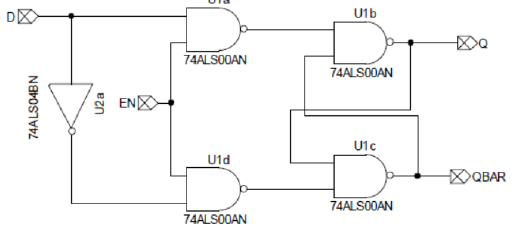
\includegraphics[scale=0.75]{../Figs-Tabs/D-Latch1.png}
		\caption{Rappresentazione di un circuito Flip-Flop D-Lantch}
			\label{f:D-Latch1}
	\end{figure}

	\begin{figure}[htb]
		\centering
		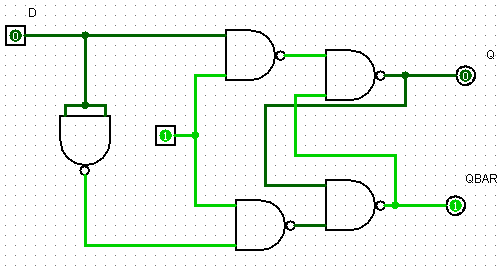
\includegraphics[scale=0.75]{../Figs-Tabs/D-Latch2.png}
		\caption{Rappresentazione del circuito Flip-Flop D-Lantch montato.
		Non disponedo di un IC SN74LS04 o analoghi la porta NOT è stata realizzata impiegando una porta NAND.}
	\label{f:D-Latch2}
	\end{figure}
	L'ingresso D del circuito è stato collegato all'ingresso Y1 dell'impulsatore basato su arduino,
	mentre l'ingresso di ENABLE è stato collegato al dip switch in dotazione.
	Si è inoltre fornita una tensione di alimentazione continua $V_{cc}\sim$\SI{5}{\volt}.

	Per la verifica del funzionamento circuitale si è andati a verificare la tabella di verità riportata in \tablename{ \ref{t:D-Lantch}}.
	\begin{table}[htb]
		\centering
		\begin{tabular}{ssss}
			\toprule
			\text{ingresso $D$} & \text{ingresso $En$ }&\text{ uscita $Q$ }&\text{ uscita $\overline{Q}$}\\
			\midrule
			0 & 0 & Q_{precedente} & {\overline{Q}}_{precedente}\\
			1 & 0 & Q_{precedente} & {\overline{Q}}_{precedente}\\
			0 & 1 & 0 & 1\\
			1 & 1 & 1 & 0\\
			\bottomrule
		\end{tabular}
	\caption{tabella di verità di un Flip-Flop D-Lantch.
	Con il pedice 'precedente' si intende che lo stato non cambi e permanga nello stato in cui si trovava indipendentemente dall'ingresso $D$.}
	\label{t:D-Lantch}
	\end{table}
	La verifica può essere effettuata con due tecniche distinte.

	Una prima qualitativa in cui si verifica la tabella di verità attraverso i diodi LED; per fare ciò si dovrebbe montare delle resistenze, per limitare la richiesta di corrente dei LED,
	rispettivamente precedentemente all'uscita $Q$ e all'uscita $\overline{Q}$.

	Ed una seconda tecnica in cui si acquisiscono le tensioni osservabili
	sulle uscite $Q$ e $\overline{Q}$ in funzione degli ingressi $D$ ed $En$.
	Essendo tale seconda  tecnica più facilmente riportabile
	si è proceduto alla verifica della tabella di verità attraverso questo metodo di verifica.

	Per fare ciò si è collegato al ingresso di $En$ all'ingresso
	$Y2$ dell'impulsatore. Essendo 	$Y1$ e 	$Y2$ sfasati di circa \ang{90}, in un periodo tali ingressi assumono tutte le possibili permutazioni di un ingresso a 2 bit.

	Si riportano le acquisizioni ottenute in \figurename{ \ref{o:D-Latch}}

	\begin{figure}[htb]
			\centering
			\subfloat[acquisizione delle tensioni in ingresso nel ciruito D-Leach; $D$ (ch1) ed $En$ (ch2)]{
				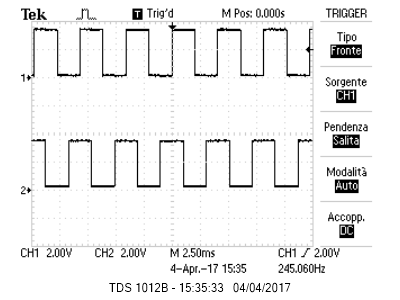
\includegraphics[scale=0.5]{../Figs-Tabs/1_input_sfasati.png}
				\label{f:ing}
			}\\
		\subfloat[acquisizione uscita $Q$ (ch1) e della tensione in ingresso $En$ (ch2)]{
			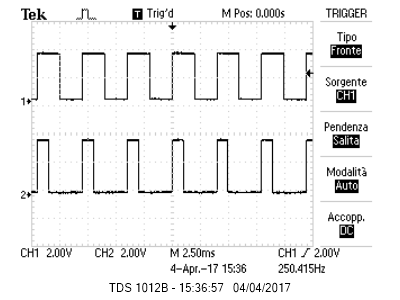
\includegraphics[scale=0.5]{../Figs-Tabs/1_data_prima.png}
			\label{f:sci}
		}
		\subfloat[acquisizione uscita $\overline{Q}$ (ch2) e della tensione in uscita  $Q$ (ch1)]{
		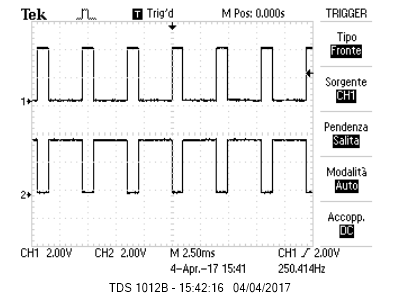
\includegraphics[scale=0.5]{../Figs-Tabs/1_q_qbarra.png}
		\label{f:sci2}
	}
		\caption{acquisizioni delle schermate impiegate per la verifica di \tablename{ \ref{t:D-Lantch}}.}
		\label{o:D-Latch}
	\end{figure}
	Dagli andamenti riportati si evince che la \tablename{ \ref{t:D-Lantch}}
	risulti verificata.
\paragraph{Misura dei tempi di ritardo}
	Essendo il circuito logico montato un sistema a più livelli
	si è assunto che i tempi di ritardo tra il segnale in ingresso e quelli in uscita non siano trascurabili.

	Si è pertanto proceduto ad una misura dei tempi di propagazione per il fronte di salita e discesa del segnale.

	Per fare ciò è stata fissata un onda quadra di frequenza $f=$\SI{250\pm 8}{\hertz} ;tale valore è stato ottenuto dal sistema di acquisizione automatica dell'oscilloscopio . Per l'incertezza associata  è stata preso il 3\textdiscount dovuta all'incertezza di calibrazione dell'oscilloscopio stesso .
	Tale onda, generata dall'impulsatore, è stata impiegata quale  segnale per l'ingresso $D$, mentre per la porta $En$ si è impiegato l'interruttore  posto normalmente sull'$1$ logico.

	Visualizzando l'andamento del segnale in $D$ e nelle uscite $Q$ e $\overline{Q}$
	sono stati misurati i seguenti ritardi:\\
	\begin{center}
		$ \Delta t_{Q,salita}=$\SI{16.4 \pm 0.1}{\nano \sec} \qquad $ \Delta t_{Q,discesa}=$\SI{29.2 \pm 0.2}{\nano \sec}\\
			$ \Delta t_{\overline{Q},salita}=$\SI{29.2 \pm 0.2}{\nano \sec} \qquad $ \Delta t_{\overline{Q},discesa}=$\SI{16.4 \pm 0.1}{\nano \sec}\\
	\end{center}

	Come è possibile osservare da i valori ottenuti $\Delta t_{\overline{Q},salita} = \Delta t_{{Q},discesa}$ e $\Delta t_{\overline{Q},discesa} = \Delta t_{{Q},salita}$; ciò risulta compatibile con le attese, essendo entrambe le uscite poste sul solito livello ed una l'inverso dell'altro.
	\paragraph{Alcune analisi sulla costituzione ciruitali }
	Come riportato in \figurename{ \ref{f:D-Latch1}} per la realizzazione del Flip-Flop D-Latch in esame si è impiegato una porta NOT;
	tale porta svolge la la funzione di inviare agli ingressi del flip-flop D-latch valori opposti; evitando pertanto di inviare in ingresso l' $1$ logico, per entrambe le porte.
	Quindi la porta NOT svolge la funzione di evitare l'ingresso del circuito nella cosiddetta zona "proibita".
	Se il sistema fosse in tale stato una successiva variazione del segnale in ingresso porterebbe a variazioni non prevedibili delle uscite.

	Si segnala inoltre che essendo le porte NAND impiegate basate su logica TTL quando esse non risultino collegate a terra si ottiene in uscita alla porta un segnale corrispondente all'$1$ logico.
	L'ingresso $En$ pertanto risulta essere attivo,e quindi abilita il circuito, per
	segnali in ingresso, in $En$, corrispondenti allo stato LOW.
